\section{Aprendizaje}  

Se entiende por aprendizaje de una red neuronal como el proceso 
por el cual se determina el valor sus pesos, es decir, lo que en el ejemplo \ref{img:Ejemplo-evaluación-red-neruonal-una-capa} consistía en las matrices $\mathfrak A$ y $\mathfrak B$. 

%%%%%%%%%%%%%%%%%%% algoritmo de gradiente descendente 

\subsection{Método de gradiente descendente y \textit{backpropagation}} \label{sec:gradiente-descendente}

De acorde a los capítulos uno y dos del libro  \cite{learning-from-data-1-2},
 una vez concretado el problema y sus elementos 
(\ref{sub:componentes_aprendizaje}) es necesario definir un método con 
el que aproximar la función ideal $f,$ para ello introduciremos el algoritmo de gradiente descendente.  

El gradiente descendente es un método iterativo de minimización de funciones diferenciables. 

% Nota sobre el algoritmo de gradiente descendente 
\reversemarginpar
\marginpar{
    \textcolor{dark_green}{    
        \textbf{
            Aclaración gradiente red neuronal
        }
    }

    Puede a priori uno confundirse con la notación,  
    pero recordemos que las redes neuronales estaban determinadas por sus parámetros (matrices), luego lo único que se está haciendo es derivar con respecto a tales parámetros.
} 
%Fin nota margen


% Idea  sobre el algoritmo de gradiente descendente 
\marginpar{
    \textcolor{dark_green}{    
        \textbf{
            Idea general del algoritmo gradiente descendente
        }
    }

    Cada iteración se obtendrá una nueva red neuronal con un error menor dentro de los datos de entrenamiento del conjunto.
} 
%Fin nota margen
En nuestro caso particular se quiere aproximar la función ideal desconocida $f$ a partir de funciones (redes neuronales) $h \in \rrnnmc$, concretamente se fijará un número $q$ de neuronas en la capa oculta. 
Dada también una función de error diferenciable y que no presente puntos de inflexión
$E: \mathcal{H}_q (\R^d, \R^s) \longrightarrow \R,$
se toma red neuronal cualquiera $h_0 \in \mathcal{H}_q (\R^d, \R^s)$ y 
fijado $\eta \in \R^+$. 

Se define la sucesión 
\begin{equation}
    h_{t+1}  = h_t - \eta \nabla E(h_t).
\end{equation}  

Donde $h_n$ es una sucesión cuyos términos convergen a un mínimo local.
\subsubsection*{Observaciones sobre el algoritmo }

\begin{itemize}
    \item El algoritmo solo encuentra óptimos locales con una dependencia crucial del valor de inicio. 
    \item La convergencia no es segura en un tiempo finito y requiere de criterios de parada. 
    \item Debe de fijarse el número de neuronas en la capa oculta a priori.
    \item Si la función es convexa el mínimo será global.
    \item El parámetro $\eta$ puede ser cualquiera y debe de ser fijado o controlado por el diseñador.  
\end{itemize}


Con el fin de reducir el coste del cálculo del gradiente, 
se utiliza el algoritmo conocido como \textit{backpropagation} que fue publicado en 
1989 en el artículo \cite{backpropagation-Hinton}. 

Denotaremos como $w$ al conjunto de parámetros que determinan el valor de una red neuronal. 

Sea $E_{in}(w)$ la función de error, la cual tomaremos como el error dentro de conjunto de entrenamiento, esto es,  si el conjunto 
de entrenamiento está constituido por $N$ datos de la forma $(x_n, y_n)$ con $x_n$ el vector de entrada y $y_n$ el estado o valor deseado para cualquier $n\in \{1, \ldots, N\}.$
\begin{equation}
    E_{in}(w) = \frac{1}{N} \sum^N_{n=1} (h_w(x)- y_n)^2. 
\end{equation}
Denotaremos como $e_n$ a 
\begin{equation}
    e_n = (h_w(x)- y_n)^2 
\end{equation}
que es una métrica para medir error entre, en nuestro caso  
la red neuronal $h_w$ y los valores de entrenamiento.

Para nuestro caso de una sola capa oculta el resultado sería el siguiente: 

El conjunto de parámetros que repercuten en la red neuronal son los de las matrices $\mathfrak{A}$ y $\mathfrak{B}$ que hemos visto que para una red $h \in \mathcal{H}_n (\R^d, \R^s)$


%% Ejemplo 
Mostraremos un ejemplo primero antes de presentar el método general para facilitar la comprensión del algoritmo. 
% Imagen red neuronal simple
\begin{figure}[h!]
    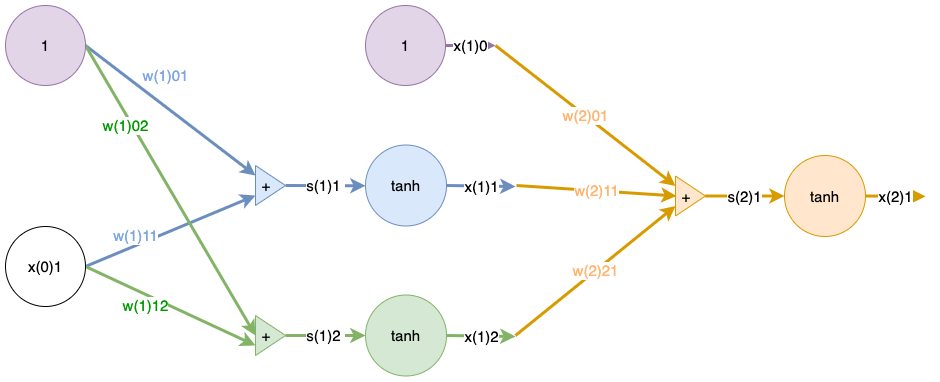
\includegraphics[width=\textwidth]{introduccion_redes_neuronales/construccion_redes_neuronales/rrnn-1-2-1.drawio.png}
    \caption{Red neuronal con una capa oculta a la que se quiere aplicar \text{backpropagation}}
    \label{img:construccion_rrnn:rrnn-1-2-1}
\end{figure} 
Queremos actualizar los pesos $w$ de la red neuronal 
$f_w : \R \longrightarrow \R$ presentada en \ref{img:construccion_rrnn:rrnn-1-2-1}.
$f_w$ está compuesta de dos capas ocultas. Supongamos que nos basaremos en un dato 
$(x, y)$ así pues podemos suponer que 
\begin{equation}
    E_{in}(w) = \frac{1}{N}e(f_w(x), y) = \frac{1}{N} (f_w(x)- y)^2.
\end{equation}
Como queremos actualizar los pesos utilizando el método de gradiente descendente necesitamos calcular el gradiente $\nabla E_{in}(w)$, en nuestro caso tenemos $w=\{W^{(1)}, W^{(2)}\}$ con 
\begin{align}
    W^{(1)} = 
    \begin{bmatrix}
        w^{(1)}_{01} & w^{(1)}_{11} \\
        w^{(1)}_{02} & w^{(1)}_{12} \\
    \end{bmatrix} 
    \text{ y }
    W^{(2)} = 
    \begin{bmatrix}
        w^{(2)}_{01} & w^{(2)}_{11} & w^{(2)}_{21}\\
    \end{bmatrix}, 
\end{align}
luego 
\begin{equation}
    \nabla E_{in}(w) = 
    \left(
        % primera capa 
        \frac{\partial e}{\partial w^{(1)}_{01}},
        \frac{\partial e}{\partial w^{(1)}_{11}},
        \frac{\partial e}{\partial w^{(1)}_{02}},
        \frac{\partial e}{\partial w^{(1)}_{12}},
        % segunda capa
        \frac{\partial e}{\partial w^{(2)}_{01}},
        \frac{\partial e}{\partial w^{(2)}_{11}},
        \frac{\partial e}{\partial w^{(2)}_{21}}
    \right).
\end{equation} 
Cada parcial se calcula, utilizando la regla de la cadena como
\begin{align}
    \frac{\partial e}{\partial w^{(1)}_{01}} 
    &=
    \frac{\partial e}{\partial s_1^{2}}
    \frac{\partial s_1^{2}}{\partial w^{(1)}_{01}} 
    \\
    &= 
    \frac{\partial }{\partial w^{(1)}_{01}}
         \tanh \left(s^{(2)}_{1}\right)
    \\
    &= 
    \left(1- \tanh^2 \left(s^{(2)}_{1}\right)\right) 
    \frac{\partial s^{(1)}_{1}}{\partial w^{(1)}_{01}}
    \\
    &= 
    \left(1- \tanh^2 \left(s^{(2)}_{1}\right)\right) 
    \frac{\partial }{\partial w^{(1)}_{01}}
    \left(w^{(2)}x^{(1)}\right)
    \\
    &= 
    \left(1- \tanh^2 \left(s^{(2)}_{1}\right)\right) 
    \frac{\partial }{\partial w^{(1)}_{01}}
    \left(
        \sum^2_{i=0}
        w^{(2)}_{i1}x^{(1)}_i
    \right)
    \\
    &= 
    \left(1- \tanh^2 \left(s^{(2)}_{1}\right)\right) 
    \left(
        \sum^2_{i=0}
        w^{(2)}_{i1}\frac{\partial x^{(1)}_i }{\partial w^{(1)}_{01}}
    \right)
    \\
    &= 
    \left(1- \tanh^2 \left(s^{(2)}_{1}\right)\right) 
    \left(
        \sum^2_{i=1}
        w^{(2)}_{i1}\frac{\partial }{\partial w^{(1)}_{01}}
        \left(
            \tanh \left(s^{(1)}_{i}\right)
        \right)
    \right)
    \\
    &= 
    \left(1- \tanh^2 \left(s^{(2)}_{1}\right)\right) 
    \left(
        \sum^2_{i=1}
        w^{(2)}_{i1}
        \left(
            \left(1- \tanh^2 \left(s^{(1)}_{i}\right)\right)
            \frac{\partial  }{\partial w^{(1)}_{01}}
            \left(
                \sum^1_{j=0}\sum^2_{k=1}
                w^{(1)}_{j k}x^{(0)}_j
            \right)
        \right)
    \right)
    \\
    &= 
    \left(1- \tanh^2 \left(s^{(2)}_{1}\right)\right) 
    \left(
        \sum^2_{i=1}
        w^{(2)}_{i1}
        \left(
            \left(1- \tanh^2 \left(s^{(1)}_{i}\right)\right)
            x^{(0)}_0
        \right)
    \right).
\end{align}
Notemos que no se han evaluado las apariciones de $s_i^{(j)}$.
Otro ejemplo sería
\begin{align}
    \frac{\partial e}{\partial w^{(2)}_{21}} 
    &=
    \frac{\partial }{\partial w^{(2)}_{21}}
         \tanh \left(s^{(2)}_{1}\right)
    \\
    &= 
    \frac{\partial }{\partial w^{(2)}_{21}}
         \tanh \left(w^{(2)}x^{(1)}\right)
    \\
    &= \left(
    1- \tanh^2 \left(s^{(2)}_{1}\right) \right)x^{(1)}_2.
\end{align}

Notemos que no se han desarrolla los términos de la forma $s^{(i)}_j$. Además si existen $Q$ pesos la complejidad del cálculo será $\mathcal{O}(Q^2)$, sin embargo, como hemos visto existen términos que se repiten en ambas ecuaciones, por lo que utilizar una técnica de programación dinámica, concretamente la conocida como 
\textit{backpropagation} (\cite{backpropagation-Hinton}) nos permite reducir el coste a una complejidad de  $\mathcal{O}(Q).$

